\documentclass[12pt]{article}
\usepackage[UKenglish]{babel} 
\usepackage{alphalph,cite}
\usepackage{amsmath}
\usepackage{amsfonts}
\usepackage{graphicx,caption}
\usepackage{floatrow}
\usepackage{xcolor}
\usepackage{wrapfig}
\usepackage{float}
\usepackage{geometry}
\usepackage{listings}
\usepackage{pdfpages}
\usepackage[onehalfspacing]{setspace}
\captionsetup{width=0.8\textwidth}
\geometry{
 a4paper,
 total={170mm,257mm},
 left=30mm,
 right=20mm,
 top=20mm,
 }
\pagestyle{headings}

\title{To what extent can a tube resonator chain model the band structure of an electron in a solid}
\author{Benjamin Cichos}
\date{\today}




\begin{document}

\section{Research Question}
To what extent can a tube resonator chain model the band structure of an electron in a solid?
\section{Introduction}  
	This investigation will discuss the analogies between quantum mechanical and acoustical phenomena. The aim of this paper is to investigate if microscopic effects as seen in quantum mechanics can be modelled by employing the propagation of wave sound in a macroscopic structure. Specifically, this is an investigation of to what extent the band structure of an electron in a solid can be modelled by conducting acoustics experiments with a tube resonator chain.	 
	
Acoustics is a subgroup of mechanics and deals with the propagation of waves through a medium, may that be a solid, liquid or gas. In this paper, however, we will solely consider acoustic waves in a gas. In a gas waves propagate as disruptions in the ambient pressure levels. The amplitude or loudness of these disturbances is related effective pressure levels as compared to a reference pressure. The distance between the compressions of a sound wave is called the wave length. The wave frequency is the number of waves that propagate past a fixed point in a given amount of time.
	
Quantum mechanics, as defined by Oxford-Dictionaries is "the branch of mechanics that deals with the mathematical description of the motion and interaction of subatomic particles, incorporation the quantisation of energy, wave-particle duality, the uncertainty principle and the correspondence principle."[7] Understanding the wave-particle duality of an electron is essential for this investigation. The electron, denoted $e^-$, is a fundamental particle that is found in orbits around neutral atoms. An electron may only assume a discrete number of allowable states in an atom, which is explained by the Schrödinger equation. For an electron to change between its allowable states it requires transfers of energy. If an electron moves to a higher-order state, it requires that additional energy be given to the electron from an external source. On the contrary, for an electron to move to a lower-order state some of its energy is expended. When atoms bond to form substances these orbitals merge, providing a greater number of allowable energy levels for the electrons to assume. When a multitude of atoms are in close proximity of each other these available energy levels form a nearly continuous spectrum wherein an electron may move. This is known as an energy band. The allowed states are still discrete, but for large number of atoms, these energy levels are so close together that they are considered to be continuous.

The reason, that effects from quantum mechanics can be investigated in acoustics, is not apparent on first sight. The basis of this correlation lies in the similarity of the Schrödinger equation with the wave equation in normal mechanics. The mathematical structure of both equations are analogous[4]. The benefit of acoustics as against quantum mechanics is that it is observable on a more appropriate time and length scale. Sound waves can easily be emitted by a loudspeaker and measured by a microphone. 

\begin{figure}[hbt]
	\caption{Electron overlap in a metallic substance}
	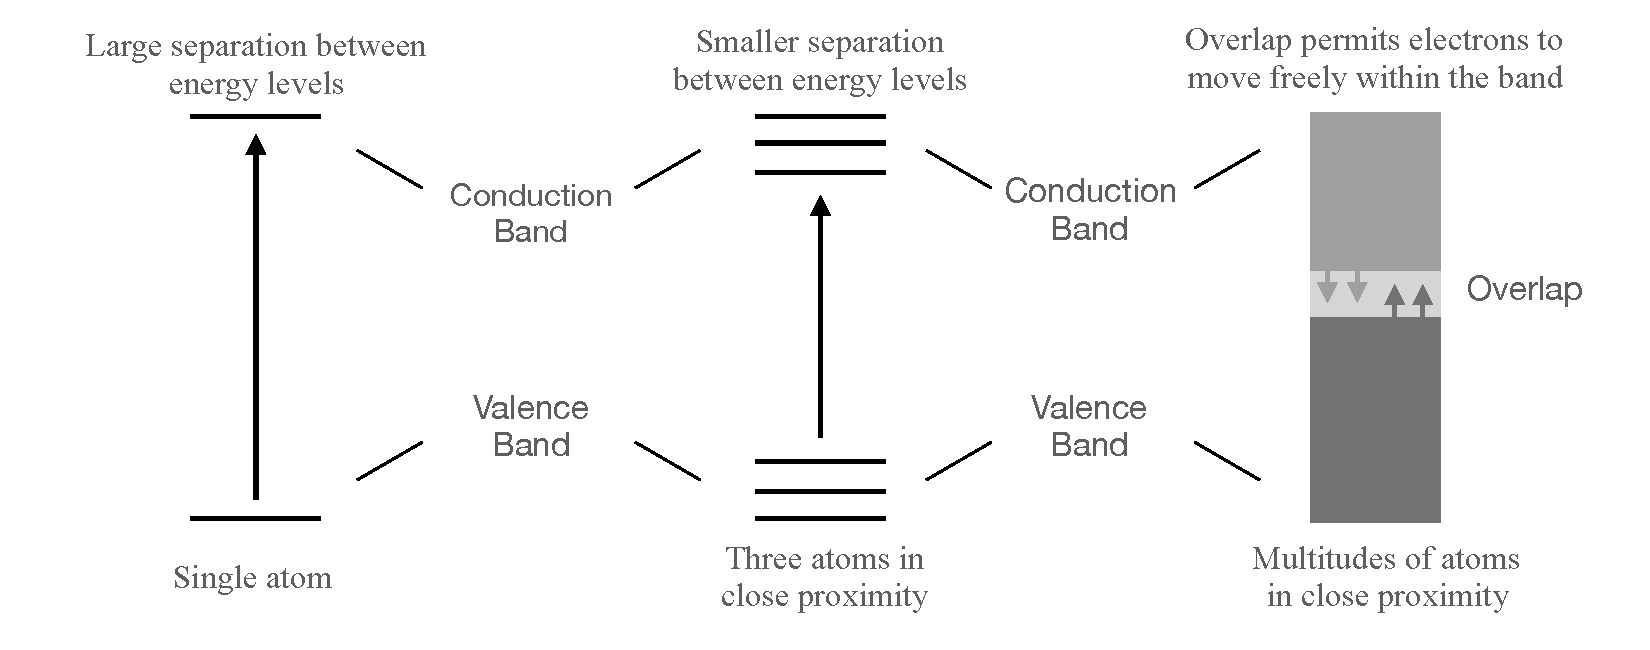
\includegraphics[width=0.8\textwidth]{introduction/band_structure}	
\end{figure}
Figure 1 illustrates the formation of an energy band in the valance band of a metallic substance. In a metallic substance the empty bands overlap with the bands containing electrons, hence, the electrons are able to move to what would normally be higher-level state without additional energy. Thus, the electrons in metallic substances are considered to be 'free' and are often described as a 'sea of electrons', due to ability to move to the conduction band without additional energy. However, this overlap is solely a characteristic of metallic substances, namely conductors. Insulators and semi-conductor are enticed by an energy gap between the valence band and the conduction band, these are known as band gaps. 
\subsection{Background Information}
For this investigation we will be examining the band structure in a solid. We assume this solid to be a crystal.
\begin{figure}[hbt]
	\caption{Scheme of a lattice structure}
	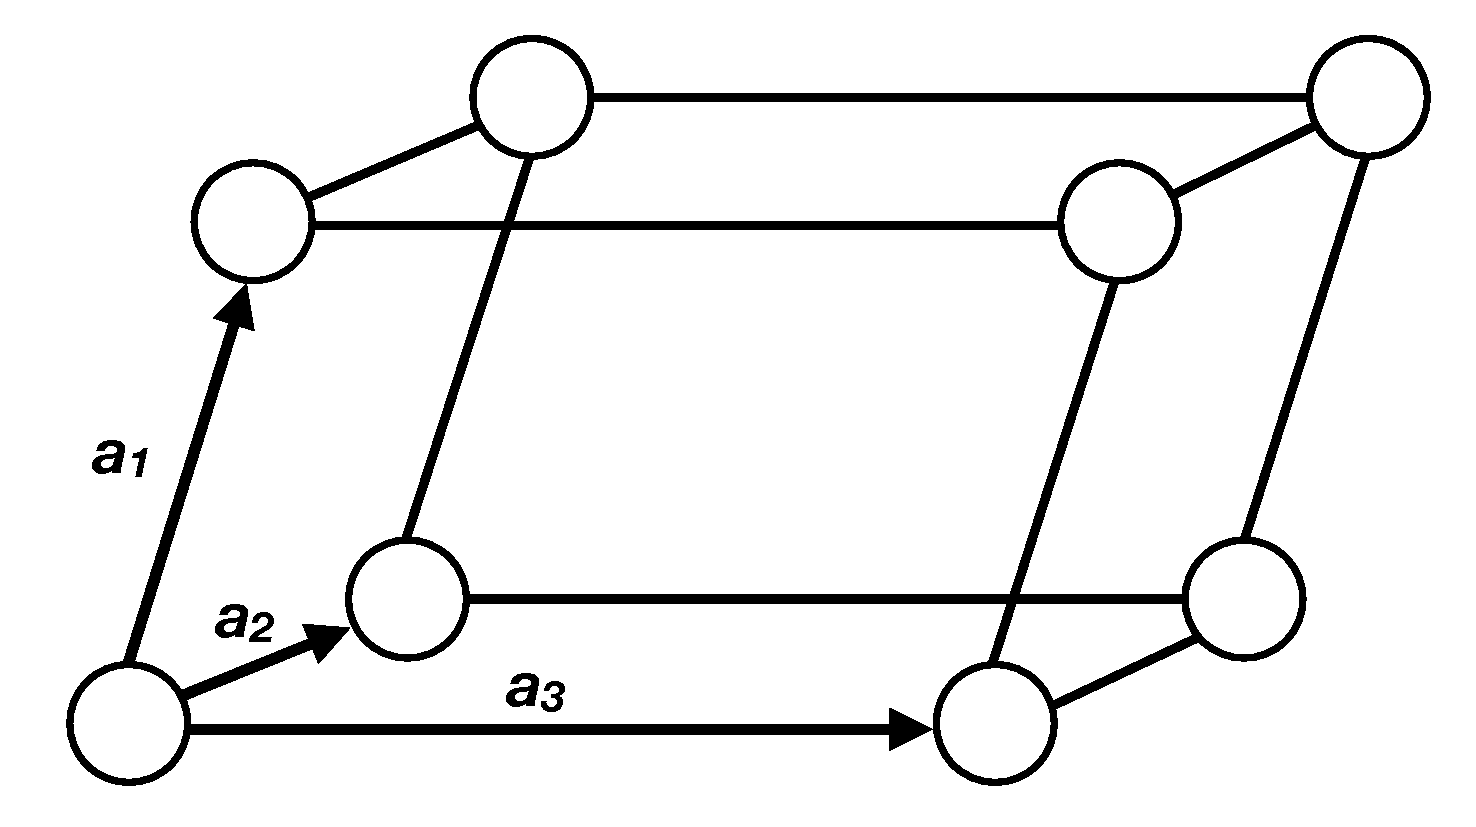
\includegraphics[width=0.5\textwidth]{introduction/crystalstructure}	
\end{figure}
A crystal is structure in which the nuclei are arranged in a strictly periodic manner, creating what is called a lattice structure. The translation of each lattice point can be written as
\begin{equation*}
	{\rm T} = m_1 a_1 + m_2 a_2 + m_3 a_3
\end{equation*}
where $a_1$, $a_2$ and $a_3$ are the lattice vectors and $m_1$, $m_2$, $m_3$ are magnitude factors. We can use the periodicity of a lattice structure and analyse the behaviour of a single electron in such a system. By examining a single electron we can disregard the interactions between electrons. To describe a periodic potential in which $V(x) = V(x+a)$, where $a$ is a lattice vector, we employ the Bloch-Theorem
\begin{equation}
	\psi (x) = u_k (x) e^{ikx}
\end{equation}
$u_k(x)$ is a periodic function, such that $u_k(x) = u_k(x+a)$. From this we can follow that
\begin{equation}
\psi(x+a) = u_k(x+a)e^{ik(x+a)} = \psi(x)e^{ika}
\end{equation}
We are able to conclude that $\psi(x+a)$ and $\psi(x)$ can only differ by a phase factor of $e^{ika}$, which is periodic, meaning that we can always choose values of $ka$ to be $-\pi < ka \leq \pi$. The value $k$ is defined as $k=\sqrt{2mE/\hbar^2}$, which is known as the wave number.
\subsubsection{Kronig-Penney-Model}
When a single electron moves through the crystal the potential increases as it approaches a nuclei and decreases as it absents itself from the nuclei. As previously mentioned, the nuclei in a crystal are periodically arranged, meaning that the potential must have periodicity also. This is illustrated in Figure 3.
\begin{figure}[hbt]
	\caption{Periodic potential in a lattice structure}
	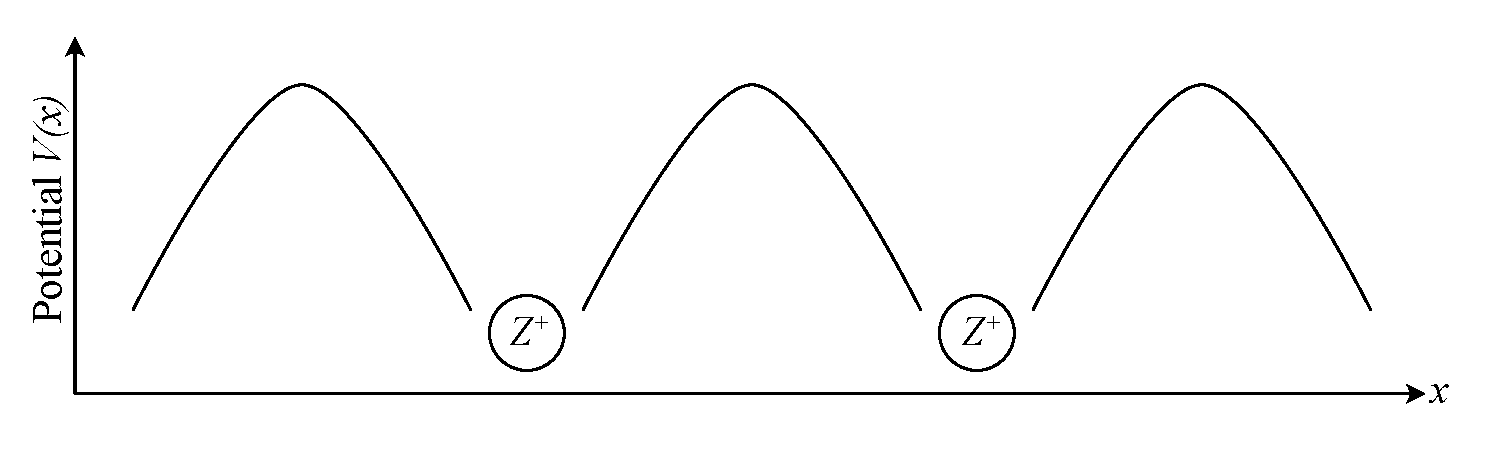
\includegraphics[width=0.8\textwidth]{introduction/periodicpotential}	
\end{figure}
\\
This was then simplified by Kronig and Penney into a periodic arrangement of potential wells and barriers. The potential wells display the region in which the electron in proximity to the nuclei and, hence, is attracted to the nuclear charge of the atom. The barriers are representational for the regions between the atoms in which the charge of nuclei is shielded by its valence electrons. The Kronig-Penney-Model is shown in Figure 4.
\begin{figure}[hbt]
	\caption{Kronig-Penney-Model of a periodic potential in a crystal. The periodicity of the potential is $V(x) = V(x+a+b)$}
	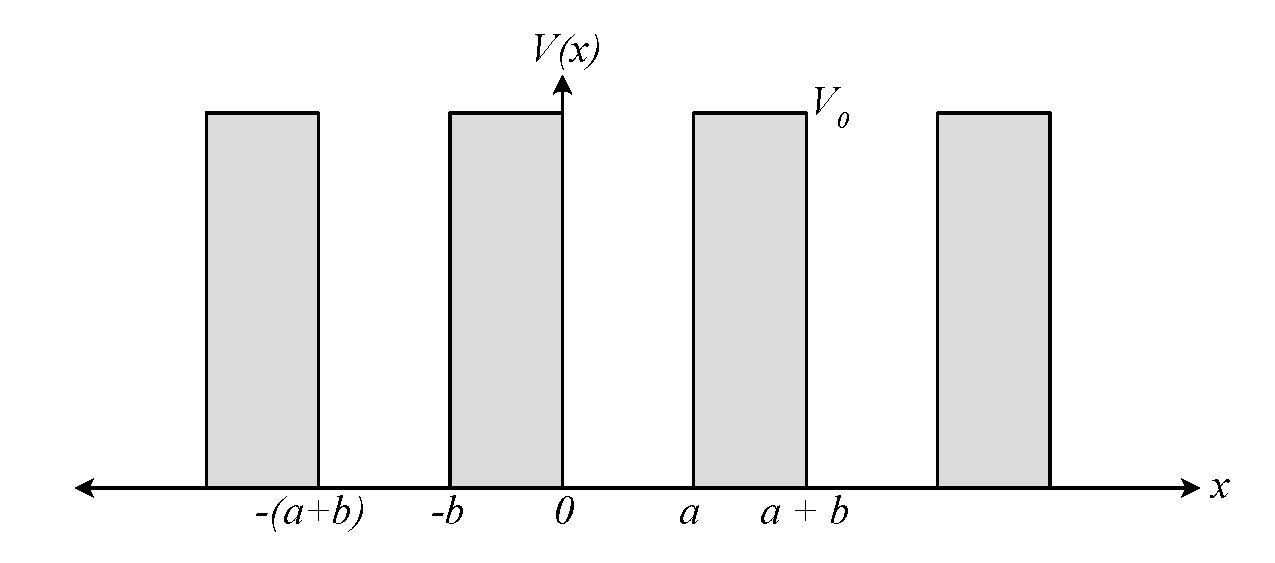
\includegraphics[width=0.8\textwidth]{introduction/kronig_penney_model.pdf}	
\end{figure}
\\
The Schrödinger-Equation of the Kronig-Penney-Model is denoted as
\begin{equation}
		\left(-\frac{\hbar^2}{2m} \frac{d^2}{dx^2} + V(x)\right)\psi(x) = E\psi(x)
\end{equation}
In the range $0<x<a$ is the solution to equation (4) given by
\begin{equation}
	\psi(x) = Ae^{i\alpha x} + Be^{-i\alpha x} \:\:\:\:\:\:\:\: where \:\:\: \alpha^2 = \frac{2m}{\hbar}E
\end{equation}
In the range $a<x<a+b$ does the solution have the form
\begin{equation}
	\psi(x) = Ce^{\beta x} + De^{-\beta x} \:\:\:\:\:\:\:\: where \:\:\: \beta^2 = \frac{2m}{\hbar}(V_0 - E)
\end{equation}
Equation (4) describes the wave function of the electron when the potential is zero. A and B are unknown coefficient that determine the forward and backward amplitude of the wave function respectively. Equation (5) illustrates the wave function when the potential is equal to $V_0$. Similarly C determines the amplitude of the forward and D the amplitude of the backward wave function. From equation (2) we can conclude that
\begin{equation}
	\psi(-b+a+b) = \psi(-b)e^{ik(a+b)}
\end{equation}
We can infer from the boundary conditions that A, B, C,  and D need to be of values, such that $\psi$ and $\frac{d\psi}{dx}$ are continuous at $x=0$ and $x=a$. At $x=0$
\begin{equation}
	A + B = C + D
\end{equation}
\begin{equation}
	i\alpha A - i\alpha B = \beta C - \beta D
\end{equation}
At $x=a$ 
\begin{equation}
	Ae^{i\alpha a} + Be^{-i\alpha a} = \left(Ce^{-\beta b} + De^{\beta b}\right)e^{ik(a+b)}
\end{equation}
\begin{equation}
	i\alpha \left(Ae^{i\alpha a}- Be^{-i\alpha a} \right) = \beta \left(Ce^{-\beta b} - De^{\beta b} \right)e^{ik(a+b)}
\end{equation}
This yields four homogenous equation for the four unknown coefficients. We can write the four equations in the matrix form.
\[
\begin{bmatrix}
	1 & 1 & -1 & -1 \\
	i\alpha & -i\alpha & -\beta & \beta \\
	e^{i\alpha a} & e^{-i\alpha a} & -e^{-\beta b}e^{ik(a+b)} & -e^{\beta b}e^{ik(a+b)} \\
	i\alpha e^{i\alpha a} & -i\alpha e^{-i\alpha a} & -\beta e^{-\beta b}e^{ik(a+b)} & \beta e^{\beta b}e^{ik(a+b)} \\
\end{bmatrix}
\begin{bmatrix}
	A\\
	B\\
	C\\
	D\\
\end{bmatrix}
=
0
\]
The solution can be obtained if the determinant of the matrix is zero. After extensive and exhausting algebra we derive the equation.
\begin{equation}
	\frac{\beta^2 - \alpha^2}{2\alpha \beta} \sinh(\beta b) \sin(\alpha a) + \cosh(\beta b) \cos(\alpha a) = \cos(k(a+b)) 
\end{equation}
We can solve equation (11) graphically, by substituting arbitrary values for $\beta$, b 
\begin{figure}[hbt]
	\caption{The function $\frac{\beta^2 - \alpha^2}{2\alpha \beta} \sinh(\beta b) \sin(\alpha a) + \cosh(\beta b) \cos(\alpha a)$. The range of $\cos(k(a+b))$ is [-1, +1].}
	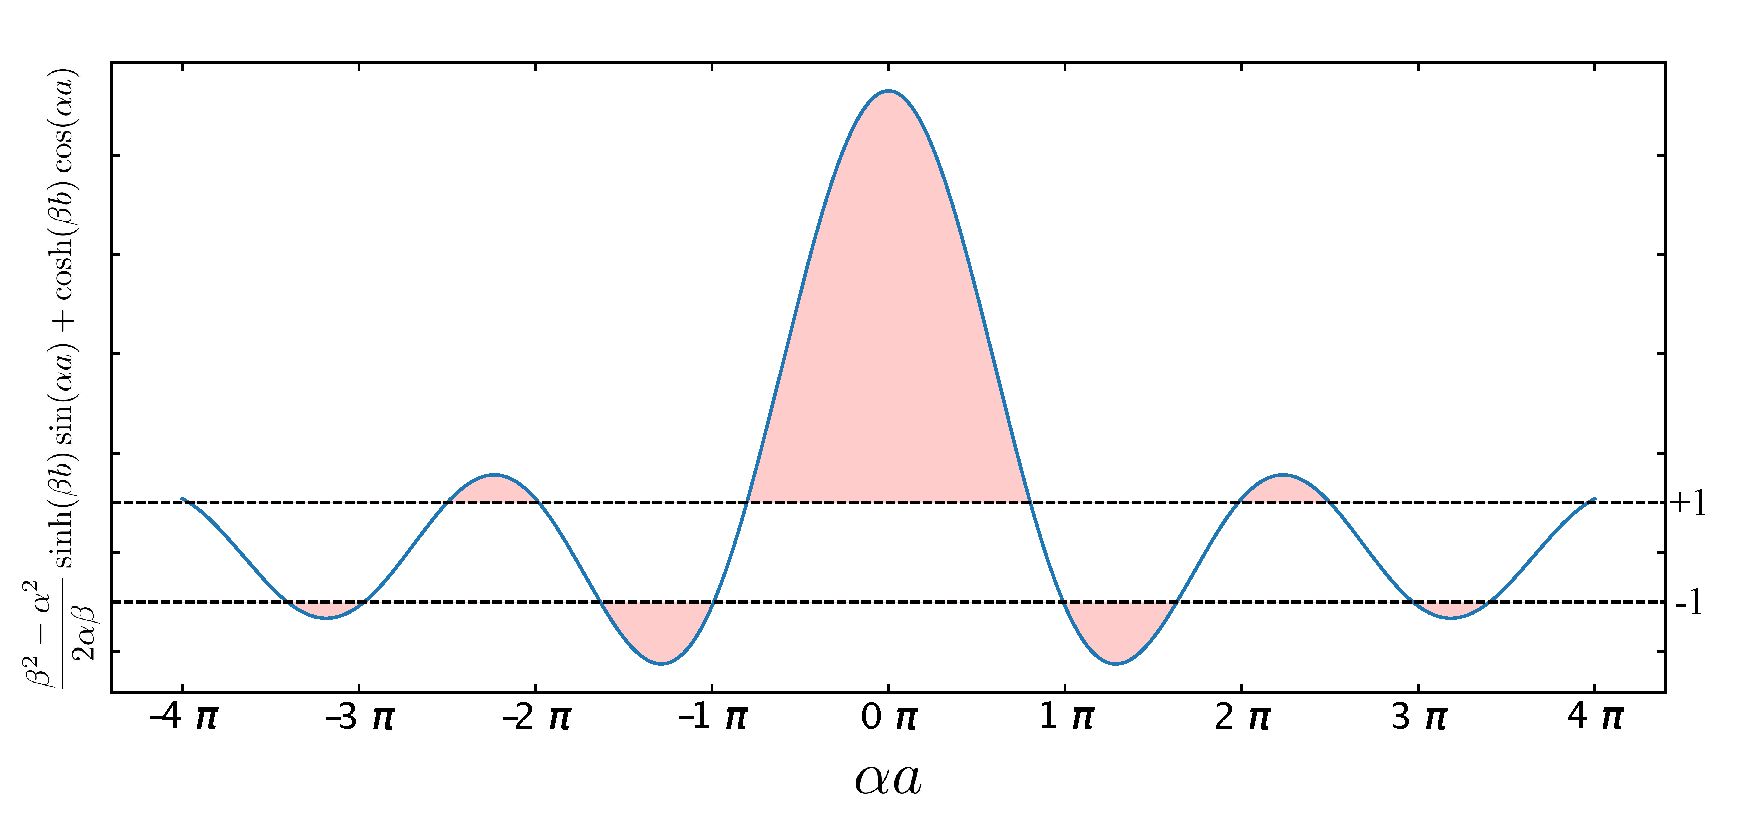
\includegraphics[width=\textwidth]{introduction/wave_number_graph}
\end{figure}
\\
Figure 5 illustrates all possible values that the wave number $k$ can assume. The solutions to the function can only exist in the range [-1, +1] as defined by $\cos(k(a+b))$. Hence, any values below or above the given states display the values that $k$ is not allowed to have. These regions are shaded in the figure for clarity. 
We determined the possible values for $k$ we can to compute the allowed energies of an electron. This is possible by employing the correlation between energy E and the wave number, that is $k = \sqrt{2mE/\hbar^2}$. This correlation is graphically presented in Figure 6.
\clearpage
\begin{figure}[hbt]
	\caption{The dispersion relation $E(k)$ of the Kronig-Penney-Model. The parabola represents the dispersion relation of a free electron. The values where $|ka|>pi$ are folded into the first Brillouin-Zone, these are marked by the blue lines.}
	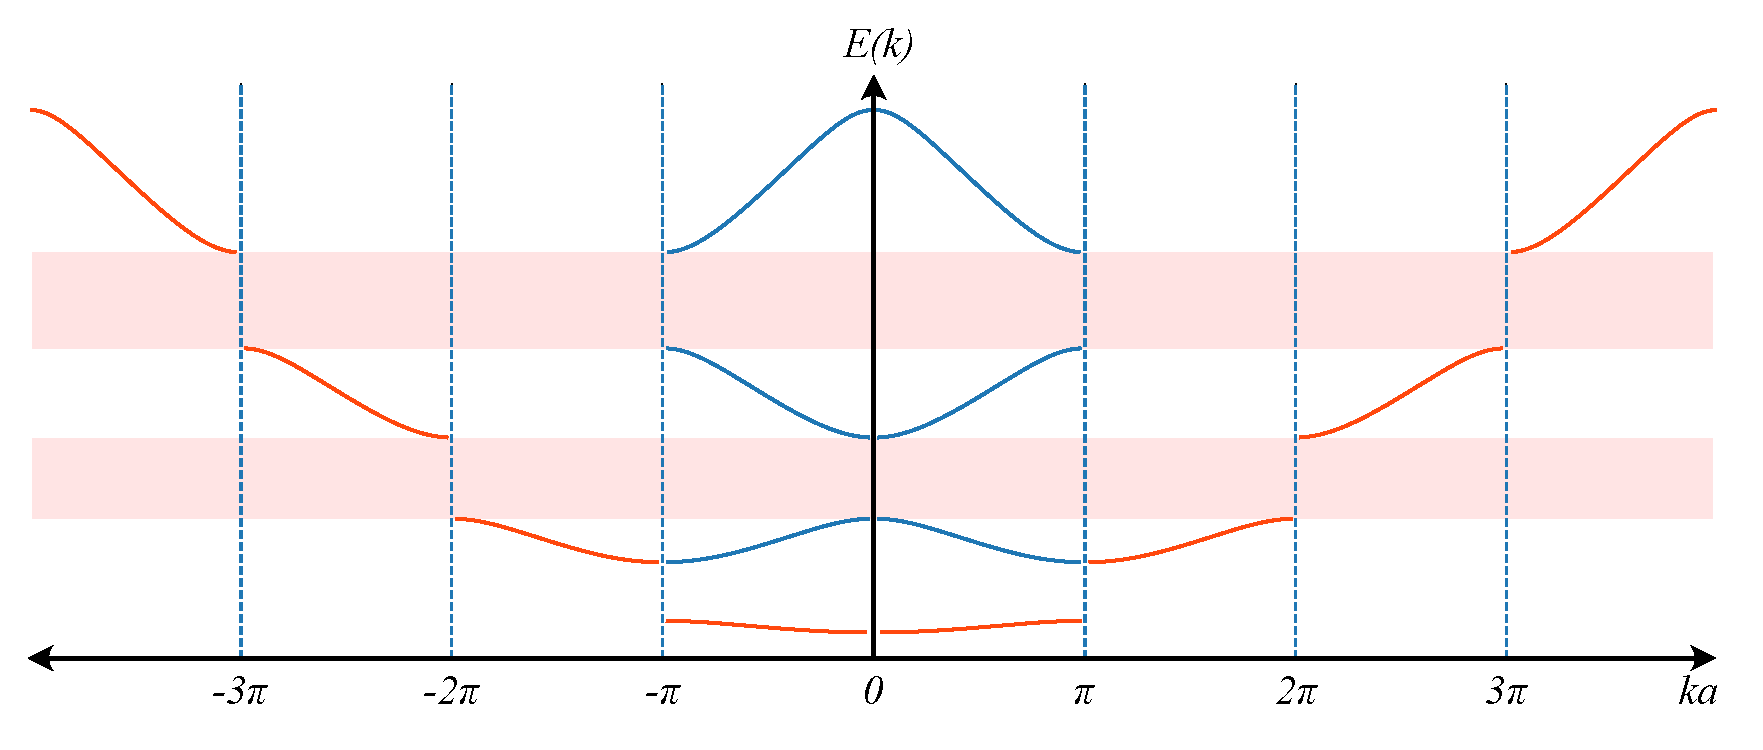
\includegraphics[width=\textwidth]{introduction/bruillon_zone}
\end{figure}
The states of the electrons are ordered in energy bands, which are separated by energy band with no allowed states. These forbidden regions are the energy band gaps. This is also known as the expanded zone scheme. In the expanded zone scheme constituted the energies of the various Brillouin-Zones. 

\subsection{Tube Resonator Chain}
\begin{figure}[hbt]
	\caption{Scheme of the tube resonator chain that consists of periodically arranged tube pieces and apertures. The apertures have a diameter of $d$ and a distance $a$ between each other. The tube resonator chain has a length of L}
	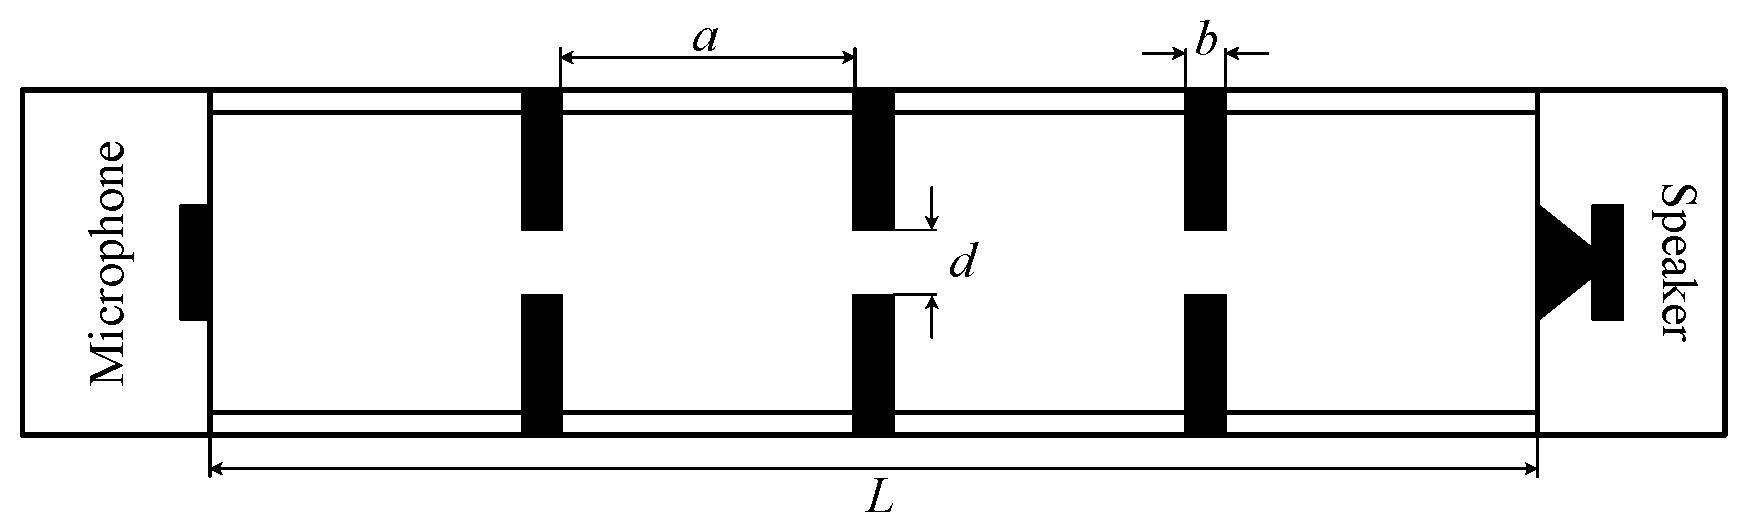
\includegraphics[width=\textwidth]{introduction/tube_resonator_chain.pdf}
\end{figure}
The tube resonator chain embodies periodically arranged apertures with a periodicity of $a$ and a diameter of $d$. It consists of $n$ tube pieces and $n-1$ apertures. The total length is $L=na + b(n-1)$. The tube is closed from both sides by a microphone and speaker, which are essential for the experiment. We will observe acoustics sound waves in the presented model of the tube resonator chain. The tube pieces acts as the potential well of the Kronig-Penney-Model, hence, one tube piece is analogous to one atoms. Therefore $n$, the number of tube pieces, effectively conveys in a quantum mechanical sense the number of atoms. The apertures are representative of the potential barrier. The diameter of the aperture is comparable to the potential $V_0$. A smaller diameter represents a larger potential and vice versa. 

\section{Variables}
\underline{\bf Independent Variable}

{\bf Length of the tube resonator chain [cm].} The length of the tube changes the density at which resonances occur. This is of relevance as the tube resonator chain has a finite length, so we can measure discrete resonances at unique frequencies, this is analogous to the discrete energy states an electron can assume. For a multitude of electrons the energy states are closer together, we examine this property in the acoustics using the length of the tube resonator chain.

{\bf Aperture.} An aperture will be introduced to the tube resonator chain. The aperture acts as a barrier for the wave propagation in the tube and is periodically arranged. This is similar to the potential barrier in a crystal. This addition of the aperture is employed to examine the formation of band structures in acoustics and its similarities to the formation of band structures in quantum mechanics.

{\bf Defect.} A defect will be inserted into the tube resonator chain. The defect is a tube piece with length $2a$, such that the apertures are no longer arranged with periodicity. Similarly, defects in a crystal also destroy its periodicity. They are localised disturbances and do not effect the band structure in a significant manner, if the density of those defects is low. We will introduce a single defect in the tube resonator chain. \\
\underline{\bf Dependent Variable}

{\bf Amplitude [Arbitrary Units].} The amplitude is measured to determine the frequencies at which the resonances occur. The resonances are analogous to the discrete energy states of an electron. The amplitude effectively displays the effects that the earlier presented independent variables have on the resonances, which are then employed for comparison to the band structure of an electron. \\
\underline{\bf Controlled Variable}

{\bf Acoustic Noise.} It is of importance that any noise from the external surroundings is minimised as much as possible. If the level of noise is too high the experiment would not be reliable as we cannot investigate the wanted frequency. The acoustic noise would interact with the frequencies propagated by the speaker unit and, hence, skew the data. To minimise noise I made sure that the environment was quiet and employed sound dampening foam. 
\section{Hypothesis}
The spacing between resonances is theorised to decrease as the length of the tube resonator chain increases. We can derive this correlation from the eqaution
\begin{equation}
	\Delta v = v_{n+1} - v_n = \frac{c}{2L}.
\end{equation}
This illustrates that as the length becomes infinitely large the distance between each resonance becomes infinitely small, such that we can no longer regard the resonances as discrete states rather we can consider them to form a continuous band. This is analogous to the phenomena in quantum mechanics that describes that electrons in an atom can only assume discrete states. However, when there is a multitude of atoms in close proximity these energy states come closer together, and we consider them to form a continuous band.

When introducing apertures to the tube resonator chain, we will observe the formation of a band structure. The bands are made up of discrete resonances, as our resonator is finite. The band gaps are the frequencies at which the sound waves are not able to propagate through the periodic structure. The apertures are comparable to the potential barrier in the lattice. In the Kronig-Penney-Model we can too observe band structures for the energies that the electron can assume. The band structure in acoustic should be harmonious to that of the electron in a crystal.

The defect will not have a distinguished effect on the band structure, which should stay the same more or less. When the defect density is low only minor changes should be seen in the band structure. Hence, we will be able to conclude that the defect an unsubstantial consequence on the whole resonator. 
\section{Experiment}
\subsection{Experimental Setup}
\begin{figure}[hbt]
	\caption{Experimental setup. a) A picture of the speaker unit. b) Tube piece of 5.0 cm length. c) Tube resonator chain consisting of 6 tube pieces. d) Aperture with 1.0 cm diameter}
	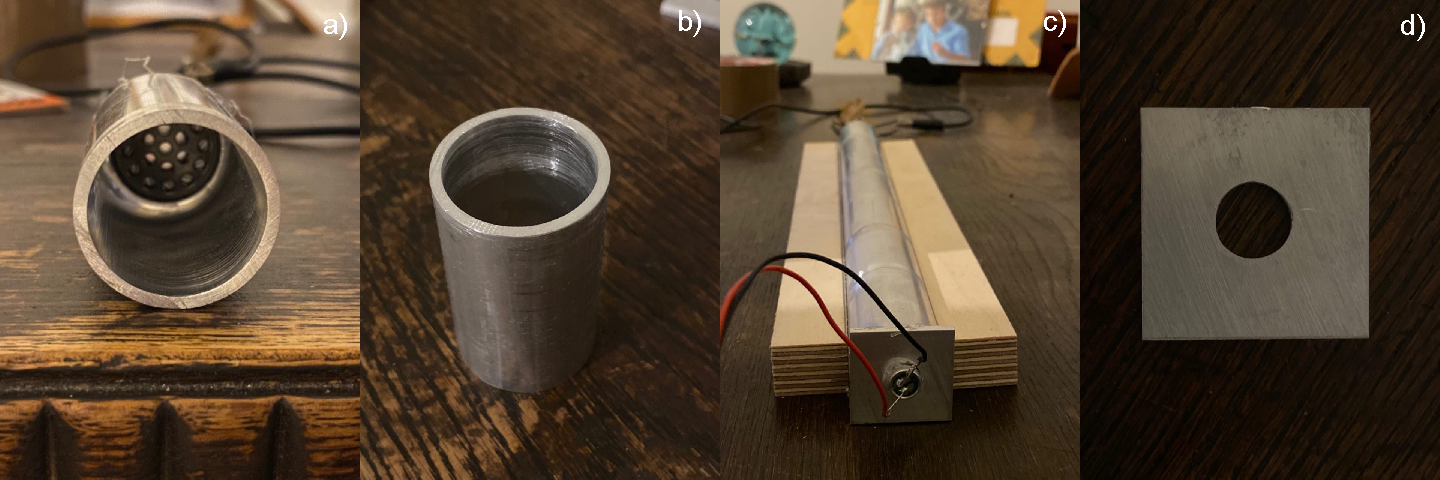
\includegraphics[width=.8\textwidth]{introduction/experimental_setup}	
\end{figure}
\subsection{Material List}
\begin{enumerate}
	\item Miniature speaker (20 - 20000 Hz)
	\item Microphone
	\item USB sound card
	\item Aluminium tube pieces (8 pieces; Length = 5.0 cm $\pm 0.001$ cm; Diameter = 30 cm $\pm 0.001$ cm)
	\item Aluminium tube defect (1 piece; Length = 10.0 cm $\pm 0.001$ cm; Diameter = 30 cm $\pm 0.001$ cm)
	\item Aluminium apertures (6 pieces; Length = 0.30 cm $\pm 0.001$ cm; Diameter = 1 cm $\pm 0.001$ cm)
	\item Computer
\end{enumerate}
\subsection{Method}
The data was acquired employing a python program. The microphone and speaker at the ends of the tube resonator chain were connected to a USB sound card which was in turn connected to a computer. A python program was running on the computer that would play frequencies, in the range 20 - 20000 Hz, through the connected speaker and simultaneously measure the frequency and amplitude by employing the microphone. The frequencies were recorded at increments of 10 Hz. The aluminium tube pieces and apertures were made by myself. The measurements of the lengths and the diameter were taken with a digital calliper that has an uncertainty of $\pm$ 0.001 cm. 
\subsubsection{Tube resonator chain without apertures}
\begin{enumerate}
	\item Construct a tube resonator chain with 6 tube pieces
	\item At the ends place the microphone and speaker unit respectively.
	\item Plug the USB sound card into the computer
	\item Connect the speaker and the microphone to the sound card
	\item Run the python program
	\item Repeat steps 1-5 with a tube resonator chain consisting of 7 and 8 tube pieces
\end{enumerate}
\subsubsection{Tube resonator chain with apertures}
\begin{enumerate}
	\item Construct a tube resonator chain with 6 tube pieces and 5 apertures 
	\item At the ends place the microphone and speaker unit respectively.
	\item Plug the USB sound card into the computer
	\item Connect the speaker and the microphone to the sound card
	\item Run the self-written python program
	\item Repeat steps 1-5 with a tube resonator chain consisting of 7 tube pieces and 6 apertures
\end{enumerate}

\subsubsection{Tube resonator chain with defect}
\begin{enumerate}
	\item Construct a tube resonator chain with 6 tube pieces (Length = 5 cm ), 1 tube defect and 6 apertures. The placement of the tube defect is not important.
	\item At the ends place the microphone and speaker unit respectively.
	\item Plug the USB sound card into the computer
	\item Connect the speaker and the microphone to the sound card
	\item Run the self-written python program	
\end{enumerate}
\subsection{Risk Assessment}
{\bf Safety Precautions:}

As I was working with technology safety precautions such as current protection are mandatory. Therefore, any liquid was kept away from any technological object such that it will not damage them. In my experiment there are no harmful substance involved, hence, normal safety precautions were taken. 
\\
{\bf Environmental Considerations:}

There are no environmental considerations to be taken into account. All of the materials used are still functional and can be employed for other purposes.
\section{Results}
\subsection{Raw Data}
The number of data points recorded exceed 1000. These are too many to represent them in a table. Table 1 illustrates a sample of the data points that were collected.
%\begin{figure}[hbt]
%	\caption{Data sample from 1110 - 1100 Hz. The tube resonator chain consists of 7 tube pieces and 6 apertures}
%	\includegraphics[width=.61901\textwidth]{table_1.pdf}
%\end{figure}

\begin{table}[hbt]
 \begin{center}
    \caption{Data sample from 1110 - 1220 Hz. The tube resonator chain consists of 7 tube pieces and 6 apertures}
    \label{tab:table4}
    \begin{tabular}{c c} 
      \hline 
     \textbf{Frequency [Hz]} & \textbf{Amplitude [a. u.]}\\
      \hline
      1110 & 868339 \\
     1120 & 901828 \\
      1130 & 1003534 \\
      1140 & 1034330 \\
      1150 & 1136530 \\
      1160 & 1118163 \\
     1170 & 1143316 \\
      1180 & 1080716 \\
      1190 & 1077889 \\
      \hline
    \end{tabular}
  \end{center}
\end{table}
The measured values are then graphed by a self-written python program to determine the frequencies at which the resonances occur.\subsection{Processed Data}
\subsubsection{Tube resonator chain without aperture}
First, we measured spectra of the tube resonator chain with length 30.0 cm, 35.0 cm and and 40.0 cm in the frequency range 20 - 20000Hz. In between the tube pieces there are no apertures. We investigate here the effect that the length of the tube resonator has on the distance between neighbouring resonances.
\begin{figure}[hbt]
	\caption{Spectra for tube resonator length of 30.0, 35.0, and 40.0 cm }
	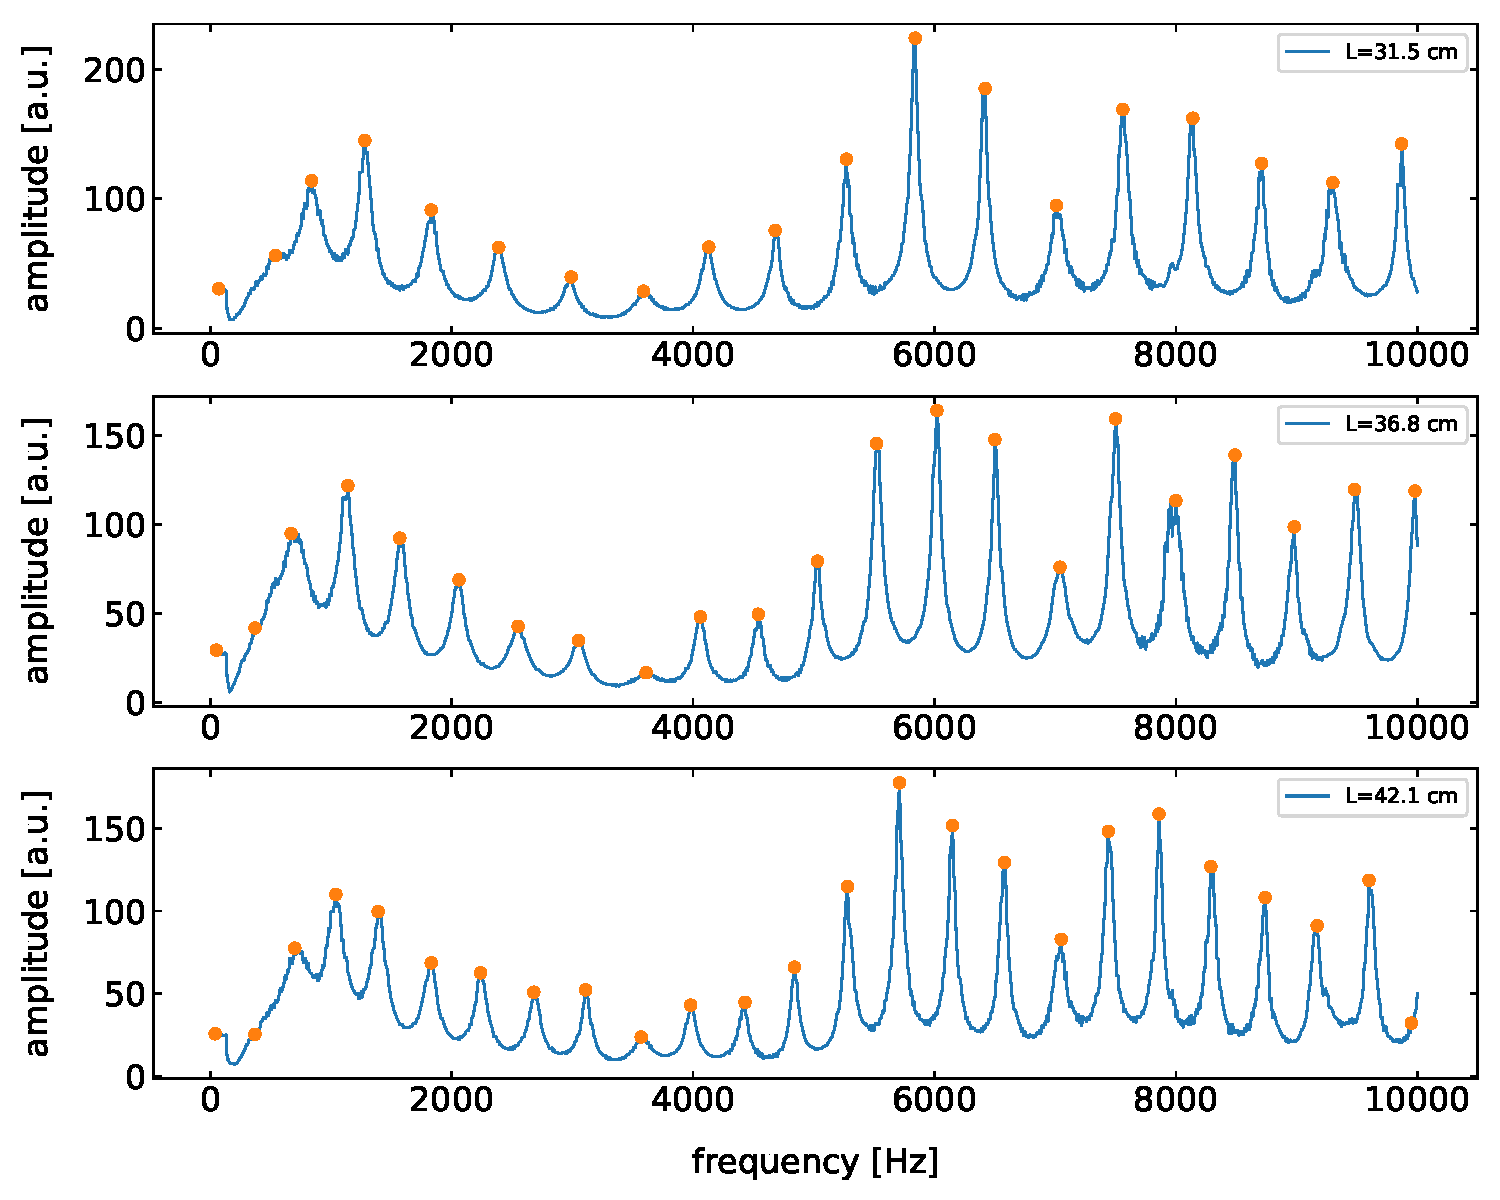
\includegraphics[width=.7\textwidth]{results/resonances_wo_aperture}	
\end{figure}
Figure 9 clearly illustrates that the density of the measured resonances increases as the tube resonator chain becomes longer. We can calculate the distance between each resonance by employing the equation $\Delta v = v_{n+1} - v_n$. From this we yield that $\Delta v$ for 31.5, 36.8, and 42.1 cm is approximately 600 Hz, 500 Hz and 440 Hz respectively. This portrays that the spacing between resonances decreases as the length of the resonator increases. The frequencies at which resonances occur in a finite resonator is given by the equation
\begin{equation}
	v_n = \frac{c}{2L}n
\end{equation}
Now, if we want to find the distance between each resonance we can rewrite this equation as
\begin{equation}
	\Delta v = v_{n+1} - v_n = \frac{c}{2L}
\end{equation}
This shows that the spacing of the resonances decreases as the length decreases. We can also predict that in resonator that is infinitely long the distances between each resonance becomes infinitely small. The resonances analogous to the discrete energy states that an electron is allowed to have. If we have a multitude of atoms in proximity these energy states come closer together, which we then regard as a continuous band. As illustrates by equation 13 resonances have a similar correlation, such that when the length is infinitely large the resonances come closer together, such that the resonances cannot be regarded as discrete states anymore rather they form a continuous band.

Energy states in quantum mechanics is given by the dispersion relation E(k). We can apply this in a similar manner to our experiment with acoustics. We can compute the wavenumber of a resonance using the equation.
\begin{equation}
	k = \frac{\pi}{L}n
\end{equation}
This shows that in a tube of a finite length we have discrete resonances, so that wave number can be derived employing the index $n$. The dispersion relation $v_n(k)$ of waves in a tube resonator is shown in Figure 10.
\begin{figure}[hbt]
	\caption{Dispersion relation $v_n(k)$ for tube resonators of length 31.5, 36.8 and 42.1 cm}
	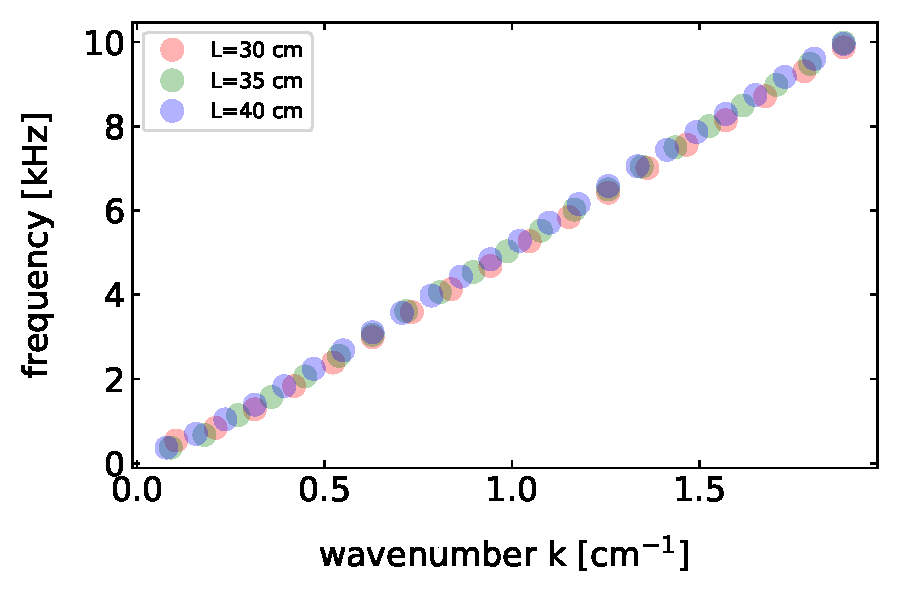
\includegraphics[width = .5\textwidth]{results/k_for_all}
\end{figure}
We can see that the proportionality between the frequency and wavenumber k remains the same for all lengths of the tube resonator chain. The only effect that the length of the resonator has is the spacing between each resonance. 


%\begin{figure}[hbt]
%	\caption{}
%	\includegraphics[width=0.7\textwidth]{k_L_315}	
%\end{figure}
%\begin{figure}[hbt]
%	\caption{}
%	\includegraphics[width=0.6\textwidth]{k_L_368}	
%\end{figure}
%\begin{figure}[hbt]
%	\caption{}
%	\includegraphics[width=0.6\textwidth]{k_L_421}	
%\end{figure}

\subsubsection{Tube resonator chain with apertures}
The second condition of the experiment is a tube resonator chain with periodically arranged apertures that have a diameter of 1 cm. The apertures are analogous to the potential barriers in a lattice structure. 
\begin{figure}[hbt]
	\caption{Spectra for tube resonator with periodically inserted apertures. The top figure shows the spectrum with length 36.8 cm or 6 tube pieces. The bottom graph for the length 42.1 cm or 7 tube pieces.}
	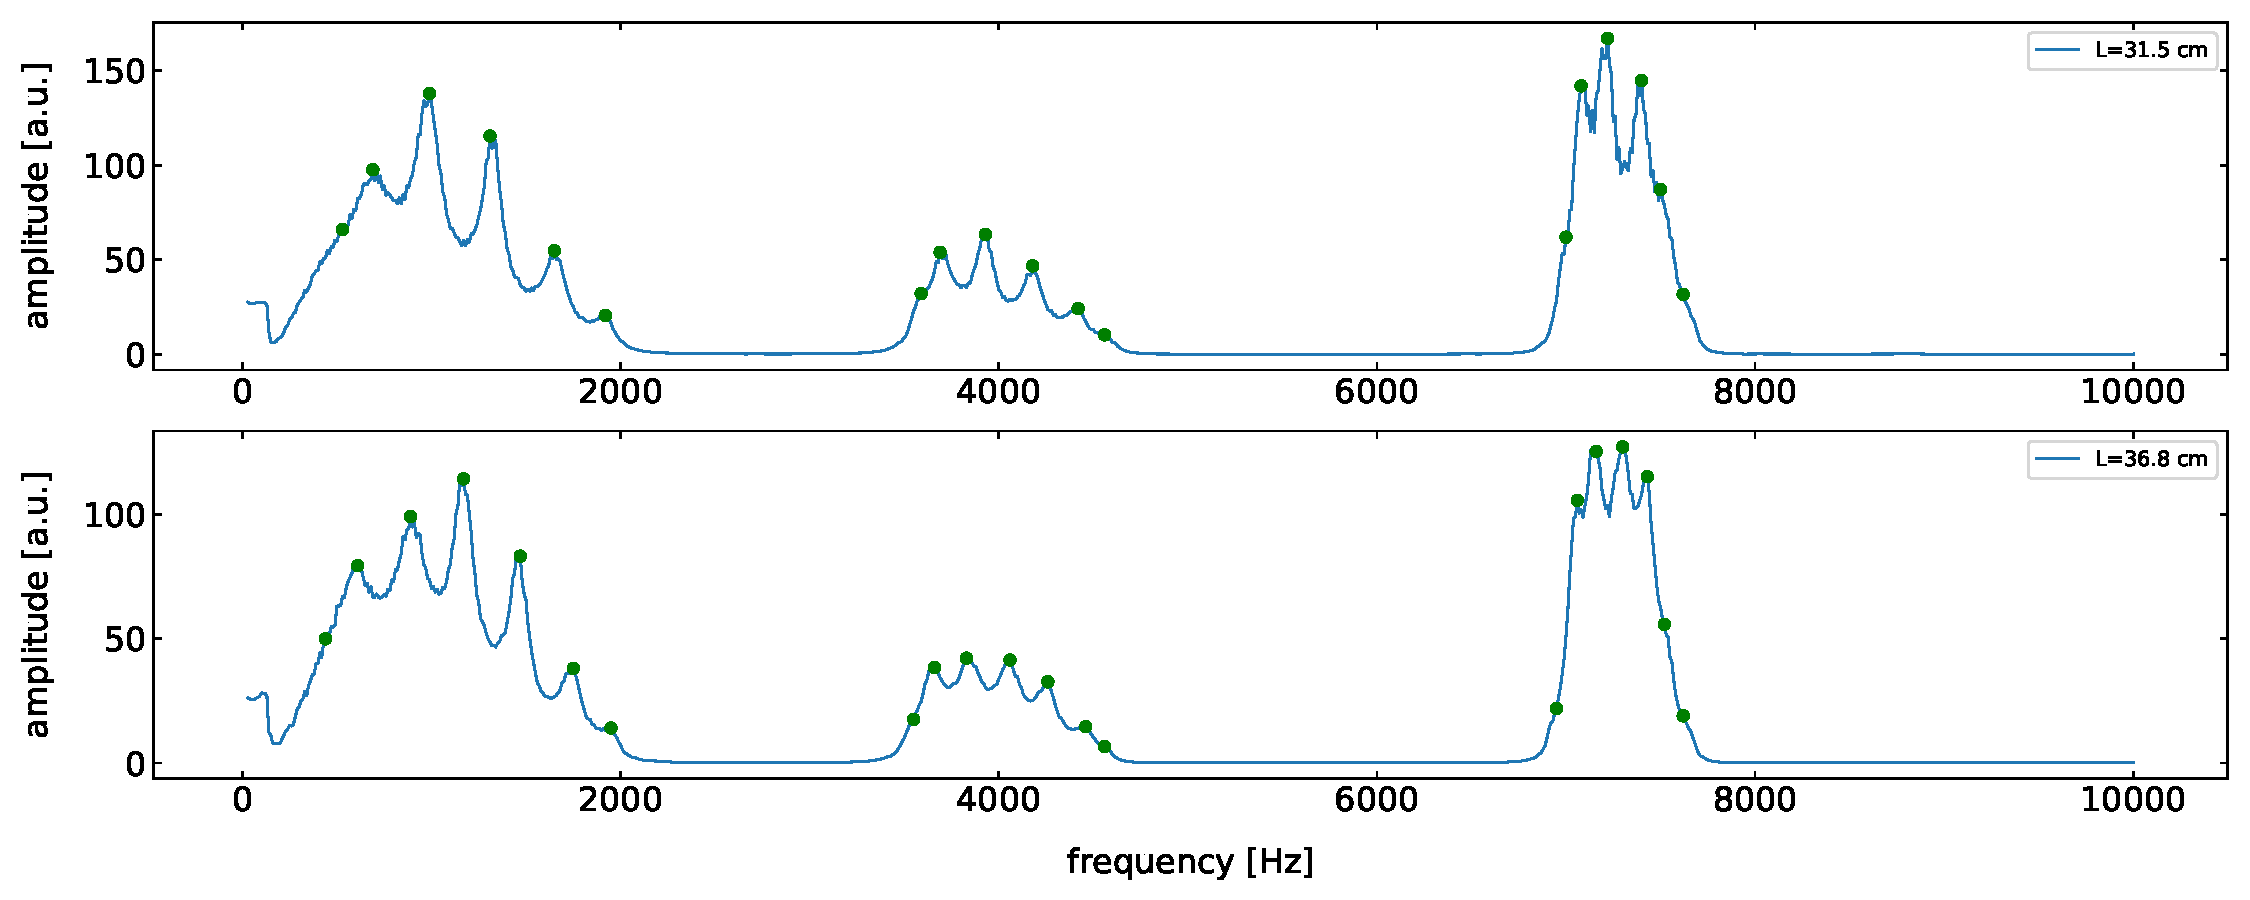
\includegraphics[width=.7\textwidth]{results/spectra_with_aperture}	
\end{figure}
Figure 12 illustrates that as apertures are introduced to the tube resonator chain we can see the formation of a band structure. Bands and bands gaps develop. The length of the tube is finite, hence, the bands consist of discrete resonances. The band gaps correspond to the frequencies at which the sound is not able to propagate through the periodic structure of the tube resonator chain.
The number of resonances in a band is determined by the number of tube pieces in the resonator. This is supported by Figure 11. Figure 12 displays the accompanying dispersion relation of the measured resonances. 
\begin{figure}[hbt]
	\caption{Dispersion relation of a tube resonator chain with apertures. The left graph shows the tube resonator of 36.8 cm. The right graph with 42.1 cm.The data points outside of the first brillouin-zone are folded back into the first zone. These are shown by the blue data points.}
	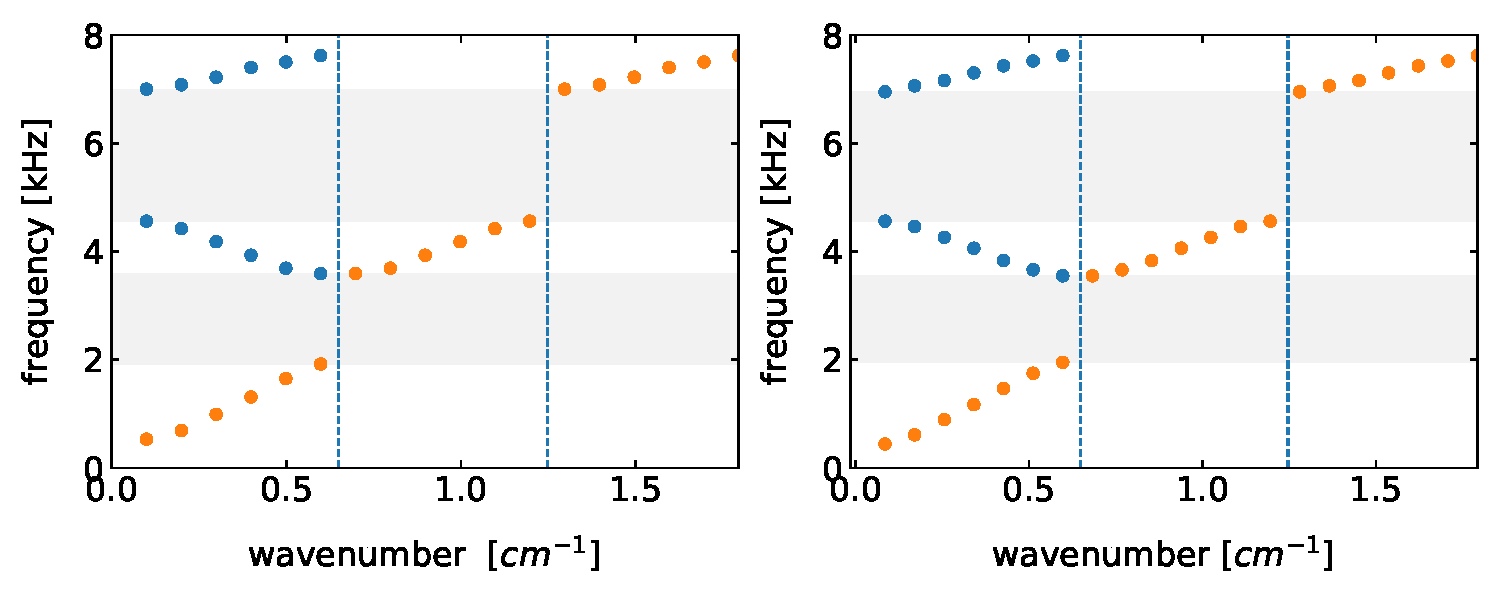
\includegraphics[width=.7\textwidth]{results/band_structure_graph}
\end{figure}
\\
Figure 12 shows that the dispersion relation of our resonances is indeed similar to the dispersion relation of an electron, as described by the Kronig-Penney-Model. 
\subsubsection{Tube resonator chain with defect}
In this section will we discuss the effect that defects have on the band structure. Defects are local disturbances that destroy the periodicity of the lattice. The defect density determines if the effect density can be seen in the band structure. When the defect density is low the band structure shows only minor changes. I investigate the effect that a single defect would have on the band structure. Figure 13 illustrates the recorded spectrum and Figure 14 shows the corresponding dispersion relation.
\begin{figure}[hbt]
	\caption{Spectrum for tube resonator chain with a defect. The defect is a 10 cm tube piece.}
	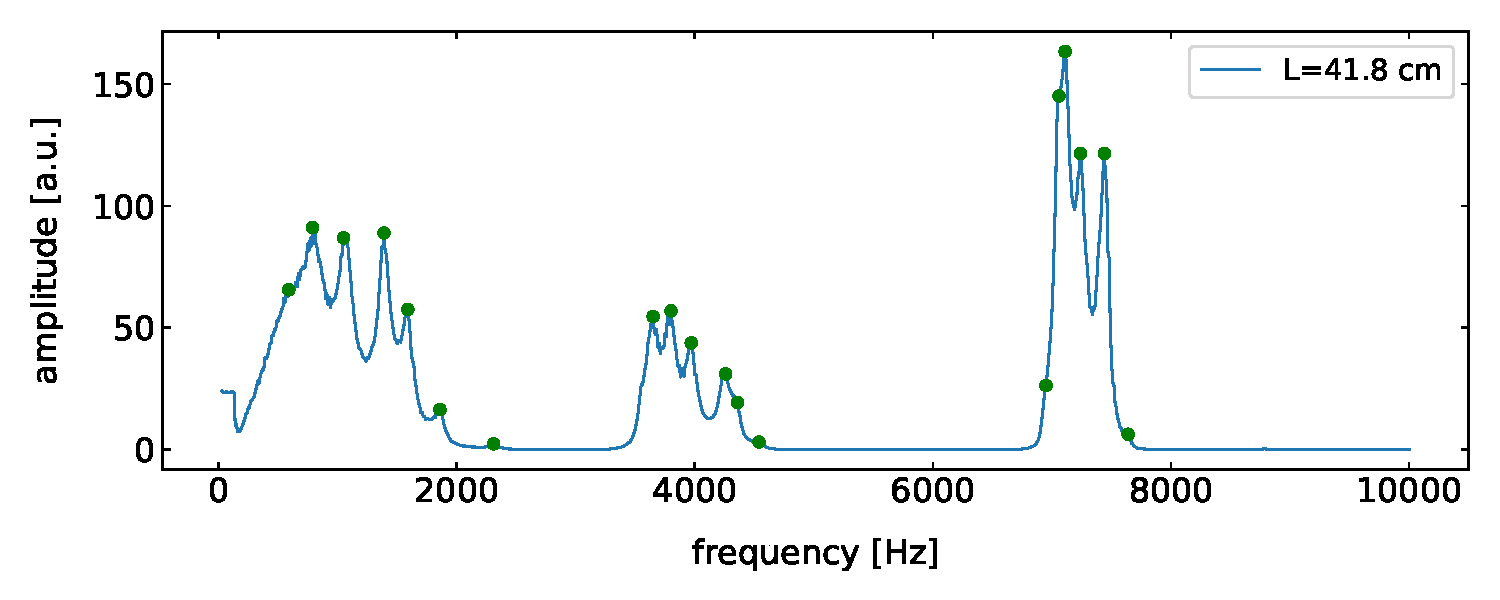
\includegraphics[width=\textwidth]{results/resonances_wi_defect}	
\end{figure}
\begin{figure}[hbt]
	\caption{Dispersion relation for tube resonator chain with a defect. The data points outside of the first brillouin-zone are folded back into the first zone. These are shown by the blue data points}
	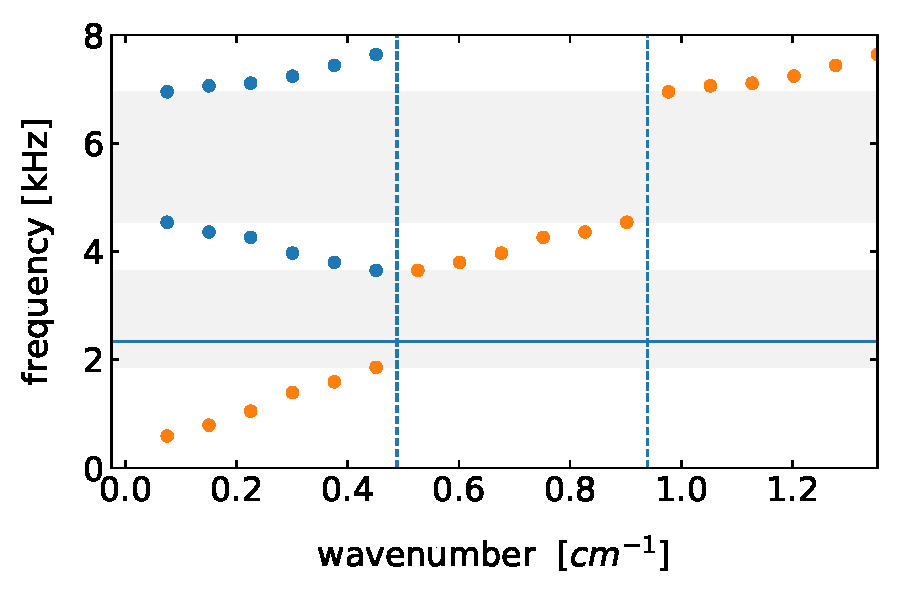
\includegraphics[width=.7\textwidth]{results/zone_with_defect}
\end{figure}
\\
The defect resonance, which we observe in the first band gap, shown in Figure 12, has a localised wave function. Since the defect resonance is localised, we cannot assign a definitive wavenumber to the resonance. Therefore, we illustrate the resonance as a horizontal line in the zone scheme. However, we see in Figure 14 that the defect has no significant effect on the band structure. The defect can be treated as a small perturbation such that we can still employ the Brillouin-Zone, which normally is only used for periodic lattices. 
\subsection{Uncertainties}
When assessing the reliability of the investigation, it is essential to examine the uncertainties. A major factor in the uncertainty of our results is the length of the tube resonator chain. We used the length of the resonator to calculate the wavenumber, hence, there is an uncertainty for our results. 

\begin{table}[hbt]
 \begin{center}
   \caption{Uncertainties in the length of the tube resonator chain}
    \label{tab:table4}
    \begin{tabular}{c c c} 
      \hline 
     \textbf{Length [cm]} & \textbf{Uncertainty in Length [cm]} & \textbf{Percentage Unc. of Length}\\
      \hline
      30.0 & $\pm 0.006$ & $\pm 0.0002\%$\\
      31.5 & $\pm 0.011$ & $\pm 0.00035\%$\\
      35.0 & $\pm 0.007$ & $\pm 0.0002\%$\\
      36.8 & $\pm 0.013$ & $\pm 0.00035\%$\\
      40.0 & $\pm 0.008$ & $\pm 0.0002\%$\\
      41.8 & $\pm 0.013$ & $\pm 0.00031\%$\\       
      \hline
    \end{tabular}
  \end{center}
\end{table}
To find the wavenumber $k$ of each resonance we employed equation (15). The other values in the equation are constants so the percentage uncertainty of the wavenumber $k$ is equal to the percentage uncertainty of the length. 
\begin{table}[hbt]
 \begin{center}
   \caption{Uncertainties in the length of the tube resonator chain}
    \label{tab:table4}
    \begin{tabular}{c c c} 
      \hline 
     \textbf{Length [cm]} & \textbf{Percentage Uncertainty of $k$} \\
      \hline
      30.0 & $\pm 0.006\%$\\
      31.5 & $\pm 0.011\%$\\
      35.0 & $\pm 0.007\%$\\
      36.8 & $\pm 0.013\%$\\
      40.0 & $\pm 0.008\%$\\
      41.8 & $\pm 0.013\%$\\       
      \hline
    \end{tabular}
  \end{center}
\end{table}
We also have an uncertainty of $\pm 0.001 cm$ in the diameter of the aperture. The diameter of the aperture is not used in any calculation, however, it is necessary to mention as the diameter affects the formation of the band structure in the resonator. 

\section{Evaluation}
\subsection{Conclusion}
The propagation of sound waves in a tube resonator chain has many similarities with the behaviour of electrons in a crystal.

When we investigated the tube resonator chain without any apertures we detected that the resonances beaome more dense as the length of the resonator increases. This means that as the resonator becomes infinitely large the spacing between each resonances becomes infinitely small. When the resonator is infinitely long we can no longer be regarded as discrete state rather we have to consider it to be a continuous band. This is analogous to the energy states an electron can assume. When there are a multitude of atoms the energy states come closer together, such that they form continuous band.

By inserting apertures between the tube pieces we create a band structure. The bands are formed by the discrete resonances; The band gaps are frequencies at which the sound waves are not able to propagate through the periodic structure. The number of pieces of pipe determines the number of resonances in each band. In principle, this also applies to the states in the solid state, but often, because of the large number of atoms (order of magnitude $10^{23}$), the states are assumed to be continuous.

When investigating an individual defect, we detect a defect resonance in the first band gap. This defect resonance has a localised wave function and therefore cannot be assigned a definitive wavenumber. However, the defect does not severely effect the band structure of the tube resonator and we are still be able to employ the Brillouin-Zone. This is comparable to the case of a defect in a crystal. The effect on the band structure is determined by the defect density in the lattice structure. If there is a single defect the band structure will remain almost unchanged.
We can, therefore, say that the propagation of sound waves effectively models the band structure of an electron in solid. 
\subsection{Strengths}
The random error of our results were relatively low. The apparatuses I used were very precise, which had the results that the random error was low in my processed data. This satisfies the reliability of the investigation. Moreover, is the quality of our data consistent. There were no recognisable anomalies in our measured data, which supports the reliability of the experiment. 
\subsection{Weaknesses}
The resonances were determined using a python code. However, the program was not able to detect all of the resonances. Hence, some of the resonances were concluded visually by hand. We can, therefore, say the detection of the resonances had an extent of inaccuracy. This might have affected the dispersion relation $v_n(k)$. This could have been improved by writing a more sophisticated python code.
The tube resonator length is due to the production of the tube pieces and due to the position of the microphone and the speaker unit afflicted with errors. Moreover, the tube resonator is made out of multiple tube pieces. The edges of the tube pieces could disturb the propagation of sound waves in the resonator. 
\subsection{Improvements and Extensions}
There are many improvement that can be made to the experiment. The quality of the tube pieces and the aperture can be improved. The tube pieces and aperture were made out of thin aluminium. If we increase the thickness and, hence, the quality of the tube pieces and apertures used we can make the investigation more reliable as this limits the vibration of the tube resonator itself. Furthermore, a wider range of lengths of the tube resonator chain should be tested to confirm the applicability of the results.

This investigation can be extended by examining how the diameter of the apertures effect the band structures formed. This is relevant as the apertures model the potential barriers in a crystal. By changing the diameter we can investigate if this changes the band structure and how this is comparable to the case for an electron in a crystal.
\section{References}
\begin{enumerate}
	\item “2.3.8. Derivation of the Kronig-Penney Model.”
	\item “Electrons in a Periodic Potential.”
	\item Fränzl, Martin. “Quantum Analogs - Akustische Experimente Zur Quantenmechanik.” Technische Universität Chemnitz, 2013.
	\item Matzdorf, Rene. “Quantum Analogs Manual.” Universität Kassel, 2009.
	\item Parajuli, Prakash. “Kronig Penny Determinant Solution.” Scribd.Parajuli, Prakash. “Kronig Penny Determinant Solution.” Scribd.
	\item “Quantum Mechanics: Definition of Quantum Mechanics by Lexico.” Lexico Dictionaries | English, Lexico Dictionaries, www.lexico.com/en/definition/quantum\_mechanics.
	\item Sokolov, Igor. “Kronig-Penney-Model.” Kronig-Penney-Modell, 14 Feb. 2005, people.physik.hu-berlin.de/~sokolov/QM1/QMall/node46.html.
\end{enumerate}
\clearpage

\end{document}